\documentclass[11pt, a4paper]{report}
\usepackage[english]{babel}
\usepackage[T1]{fontenc}
\usepackage[utf8]{inputenc}
\DeclareUnicodeCharacter{2010}{-}% support older LaTeX versions
\usepackage{wallpaper}
\usepackage{palatino}
\usepackage{changepage}
\usepackage{mhchem} % for isotope nomeclature support
% Setup captions
%\captionstyle[\centering]{\centering}
%\changecaptionwidth
%\captionwidth{0.8\linewidth}

% Protect against widows and orphans
%\clubpenalty=10000
%\widowpenalty=10000

%\linespread{1.2}

%\raggedbottom

%\chapterstyle{ger}

%\maxsecnumdepth{subsection}

%%  Setup fancy style quotation
%%  ==================================================================
%\usepackage{tikz}
%\usepackage{framed}

%\newcommand*\quotefont{\fontfamily{fxl}} % selects Libertine for quote font

% Make commands for the quotes
%\newcommand*{\openquote}{\tikz[remember picture,overlay,xshift=-15pt,yshift=-10pt]
%     \node (OQ) {\quotefont\fontsize{60}{60}\selectfont``};\kern0pt}
%\newcommand*{\closequote}{\tikz[remember picture,overlay,xshift=15pt,yshift=5pt]
%     \node (CQ) {\quotefont\fontsize{60}{60}\selectfont''};}

% select a colour for the shading
%\definecolor{shadecolor}{rgb}{1,1,1}

% wrap everything in its own environment
%\newenvironment{shadequote}% 
%{\begin{snugshade}\begin{quote}\openquote}
%{\hfill\closequote\end{quote}\end{snugshade}}



%% MY STUFF


%% Language and font encodings

%% Sets page size and margins
%\usepackage[a4paper,top=2.5cm,bottom=2cm,left=2.5cm,right=2.5cm,marginparwidth=1.75cm]{geometry}
\usepackage{graphicx}
\graphicspath{{./plots/}{./figures/}}

%\fancypagestyle{title}{%
%  \setlength{\headheight}{120pt}%
%  \fancyhf{}% No header/footer
%  \renewcommand{\headrulewidth}{0pt}% No header rule
%  \renewcommand{\footrulewidth}{0pt}% No footer rule
%  %\fancyhead[L]{\small\begin{tabular}{@{}l}\includegraphics[width=0.15\textwidth]{ku}\end{tabular}}
%   % \fancyhead[C]{\small\begin{tabular}{@{}l}\includegraphics[width=0.6\textwidth]{PROSCION}\end{tabular}}
%  %\fancyhead[R]{\small\begin{tabular}{@{}r}\includegraphics[width=0.15\textwidth]{naturvidenskab}\end{tabular}}
%}%


%\usepackage{amsmath}
%\usepackage[format=plain]{caption}
\usepackage{subcaption}
\usepackage{float} % force float
\usepackage[nottoc,numbib]{tocbibind} % make bibliography appear in toc
%\usepackage[margin=-50pt]{caption}
%\usepackage[colorinlistoftodos]{todonotes}
\usepackage[colorlinks=true, allcolors=blue]{hyperref}
\usepackage{cleveref} % for enumerate/itemize item referencing

%\setlength{\parindent}{4em}
%\setlength{\parskip}{1em}
%\usepackage{mathpazo} % Use the Palatino font
\usepackage{parskip}% http://ctan.org/pkg/parskip
\usepackage{xspace}
\usepackage{wrapfig}
\usepackage[export]{adjustbox}
\usepackage{textcomp}
\usepackage[bottom]{footmisc}


\usepackage{titling}
\newcommand{\subtitle}[1]{%
  \posttitle{%
    \par\end{center}
    \begin{center}\large#1\end{center}
    \vskip0.5em}%
}

\renewcommand\thesubfigure{\arabic{subfigure}}  
\captionsetup{format=hang,labelsep=space,indention=-2cm,labelfont=bf,width=.9\textwidth,skip=.5\baselineskip}
%\captionsetup[sub]{labelfont=bf, labelsep=period,labelformat=simple, subrefformat=brace}


\usepackage{listings}
\lstset{basicstyle=\ttfamily,
  showstringspaces=false,
  commentstyle=\color{red},
  keywordstyle=\color{blue}
}

\makeatletter
\renewcommand\p@subfigure{\thefigure\,}
\renewcommand\thesubfigure{\alph{subfigure})}
% If desired for table as well:
% \renewcommand\p@subtable{\thetable\,}
% \renewcommand\thesubtable{\alph{subtable})}
\DeclareCaptionLabelFormat{mysublabelfmt}{\alph{sub\@captype}}
\makeatother

\renewcommand{\baselinestretch}{1.5}
\DeclareCaptionSubType*[arabic]{figure}



%\makeatletter
%\renewcommand\thesection{}
%\renewcommand\thesubsection{\@arabic\c@subsection}
%\makeatother

\usepackage{mathtools}

\DeclarePairedDelimiter\abs{\lvert}{\rvert}%
\DeclarePairedDelimiter\norm{\lVert}{\rVert}%

% Swap the definition of \abs* and \norm*, so that \abs
% and \norm resizes the size of the brackets, and the 
% starred version does not.
\makeatletter
\let\oldabs\abs
\def\abs{\@ifstar{\oldabs}{\oldabs*}}
%
\let\oldnorm\norm
\def\norm{\@ifstar{\oldnorm}{\oldnorm*}}
\makeatother

\usepackage{acro}
\acsetup{first-style=short}

\DeclareAcronym{MS}{
  short = MS ,
  long  = Mass Spectrometry,
  class = abbrev
}

\DeclareAcronym{MS1}{
  short = MS1 ,
  long  = first tandem MS analyzer ,
  class = abbrev
}

\DeclareAcronym{MS2}{
  short = MS2 ,
  long  = second tandem MS analyzer ,
  class = abbrev
}

\DeclareAcronym{MS/MS}{
  short = MS/MS ,
  long  = Tandem mass spectrometry,
  class = abbrev
}


\DeclareAcronym{m/z}{
  short = m/z ,
  long  = mass charge ratio,
  class = abbrev
}

\DeclareAcronym{MALDI}{
  short = MALDI ,
  long  = Matrix-Assisted Laser-Desorption Ionization,
  class = abbrev
}

\DeclareAcronym{ESI}{
  short = ESI ,
  long  = Electrospray Ionization,
  class = abbrev
}


\DeclareAcronym{TOF}{
  short = TOF ,
  long  = Time of Flight,
  class = abbrev
}

\DeclareAcronym{IT}{
  short = IT ,
  long  = Ion Trap,
  class = abbrev
}

\DeclareAcronym{Q}{
  short = Q,
  long  = Quadrupole,
  class = abbrev
}

\DeclareAcronym{FT-ICR}{
  short = FT-ICR ,
  long  = Fourier Transform Ion Cyclotron Resonance,
  class = abbrev
}


\DeclareAcronym{HPLC}{
  short = HPLC ,
  long  = High pressure liquid chromatography,
  class = abbrev
}



%%  Begin document
%%  ==================================================================
\begin{document}

%%  Begin title page
%%  ==================================================================
    \thispagestyle{empty}
    \ULCornerWallPaper{1}{nat-farve.pdf}
    \ULCornerWallPaper{1}{nat-en.pdf}
    \begin{adjustwidth}{-3cm}{-1.5cm}
    \vspace*{-1cm}
    \textbf{\Huge Bioinformatics Master Thesis} \\
    \vspace*{2.5cm} \\
    \textbf{\Huge Topics in Mass Sectrometry and Proteomics} \\
    \vspace*{.1cm} \\
    %{\huge No subtitle is available} \\
    \begin{tabbing}
    % adjust the hspace below for the longest author name
    Antonio Ortega Jiménez \hspace{1cm} \= \texttt{<ntoniohu@gmail.com>}
    %Second Author \> \texttt{<second@author.com>} \\       
    \\[10.5cm] 
    
    \textbf{\Large Supervisors} \\
    Thomas Hamelryck \> \texttt{<thamelry@gmail.com>} \\
    Mathias F. Gruber \> \texttt{<mafg@novozymes.com>} \\

    \end{tabbing}
    \end{adjustwidth}
    \newpage
    \ClearWallPaper
%%  ==================================================================
%%  End title page

%%%%%%%%%%%%% Indholdsfortegnelse %%%%%%%%%%%%%
\setcounter{tocdepth}{1}
\tableofcontents % Indholdsfortegnelse
%\listoffigures   % Liste over figurer \begin{figure} ... \end{figure}
%\listoftables    % Liste over tabeller \begin{table} ... \end{table}
%%%%%%%%%%%%%%%%%%%%%%%%%%%%%%%%%%%%%%%%%%%%%%%

\thispagestyle{empty}
\printacronyms[include-classes=abbrev,name=Abbreviations]

\newpage
\setcounter{page}{1}


\section*{Preface}

\chapter{Introduction}
\label{chap:introduction}

\section{Aminoacids and proteins}

Proteins represent the last link in the central dogma of biology, where information encoded in DNA, is transcribed to RNA for posterior translation into proteins at the ribosome.

Proteins are made up of 20 basic units, called aminoacids. All aminoacids share a common chemical structure, where a carbon atom ($C_\alpha$) is covalently bonded to a hydrogen atom, a carboxyl group, an amino group, and last but not least, a radical, also called side chain of the aminoacid (see figure \ref{fig:aminoacids}. The side chain differs between aminaocids and generates them from each other. A slight deviation from this pattern exists in proline, where the radical is bound to the nitrogen atom, making it an iminoacid. Even though the side chains are all different, they can be classified into four different groups: aliphatic, polar, positively charged and negatively charged (see figure \ref{fig:aminaocids}).

\begin{figure}
  \centering
  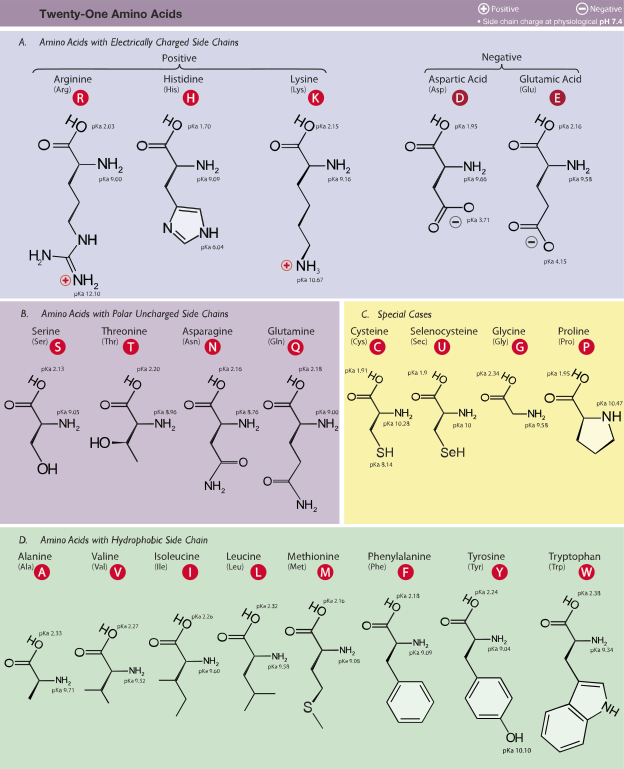
\includegraphics[width=0.5\textwidth]{aminoacids.png}
  \caption{}
  \label{fig:aminaocids}
\end{figure}

Two aminoacids are joined together through the formation of a peptidic (covalent) bond between them. Such a linkage is formed by removal of the elements of water (dehydration) from the $\alpha$-carboxyl group of one amino acid and the $\alpha$-amino group of another. CITE LEHNINGER PAG 82. The remaining $\alpha$-amino and $\alpha$-carboxyl groups are available for linkage to other aminoacids, and in this way peptidic chains or peptides can be created.

While there are 20 basic units that constitute the majority of naturally observable proteins, their side chains can be modified both by physiological processes and by experimental procedures CITE. One frequent instance of such modifications is the oxidation of methionine


\section{The protein-focused biotechnology industry}


Proteins carry out most of the cell\textquotesingle s molecular functions, they work as molecular agents that can perform an extremely wide range of tasks. The advent of biotechnology has sought to take advantage of this power, either by using proteins as present in natural conditions (wild type) or engineered by humans. This potential economic activity is carried out by several biotech companies, including Novozymes.

Novozymes A/S is a company whose line of business consists of the development of enzymatic products performing chemical transformations in different industrial processes. The application of these products, instead of conventional chemical-based solutions, has the advantage that they require less chemical substances, potentially simplifying industrial processes, reducing their costs and their environmental impact. Notorious examples of such applications include waste-water treatment, household care and the baking industry.

In order to place Novozymes ahead of its competitors, the company has utmost interest in developing protein research and several departments in the organization approach the study of proteins and their translation to the market through among other things the application of Mass Spectrometry (\ac{MS}) and Proteomics.

\section{Objectives of the Thesis}
\label{sec:objectives}

In line with the goal of making Novozymes more competitive, this project aimed at the following objectives:

\begin{enumerate}

\item Develop an open-source, Linux based and straightforward to deploy pipeline for the analysis of mass spectrometry data, starting at the output RAW files and ending in the interpretation of the results.

\item Evaluate this pipeline with a benchmark dataset to assess if the pipeline is able to reflect the biological phenomena captured in the data.

\item Implement a label-free quantification Bayesian-based method using Pymc3.

\end{enumerate}



\chapter{Mass spectrometry and shotgun proteomics}
\label{chap:mass_spec}

Life systems consist of complex systems, meaning their behaviour cannot be easily explained by analyzing the individual elements alone. Moreover, they present multiple layers of complexity, given by the nature of the elements that make it up. The layer provided by proteins is one of them, and its study is called proteomics. It is a complex layer because thousands of different proteins can be present in a single cell at any time, and their exact composition and quantities constantly change, responding to the stimuli of the surrounding environment. The study of the protein-specific complexity is called proteomics. With proteomics, one endeavors to infer the protein composition of a sample, and eventually quantify its protein amounts.

It may be useful to divide the existing approaches into two types of paradigms: top-down and bottom-up. In the top-down paradigm, intact proteins are directly used for the analysis. In the bottom-up paradigm, the proteins are first cleaved into smaller parts, and these parts are then used for identification, characterization, and quantification. These smaller parts are called peptides. CITE 1.6.1 COMPUTATIONAL METHODS. Such peptides acquire physicochemical properties fitting the requirements of the downstream analytical methods, mainly mass spectrometry (MS), which performs the data acquisition. The bottom-up paradigm is most often used because peptides are much more suitable to analysis by mass spectrometry. The interested reader is directed to CITE 1.6.1 COMPUTATIONAL METHODS to learn why. The top-down paradigm will be ignored in the rest of the manuscript.

MS is performed by means of a mass spectrometer, an ensemble of pieces of equipment that can acquire mass measurements for plenty of sample components. A detailed explanation of the sample processing required prior to MS is given in section \label{sec:sample processing}, while an overview on mass spectrometers is given in section \label{sec:the mass spectrometer}. The result of the MS analysis is a dataset that, with adequate computational analysis tools, is enough to perform the inference steps required to gather knowledge about the original protein sample. These inference steps can be condensed to the peptide and protein inference problems, explained in section \label{sec:peptide and protein inference}. A third computational problem needs to be solved if quantitative, and not just qualitative information, is to be gained from the experiment. This is the quantification problem, explained in section \label{sec:quantification} CITE.

A summary of the bottom-up approach MS analytical pipeline follows.


\section{Sample processing}
\label{sec:sample_processing}

An \ac{MS} experiment starts with the generation of protein mixture samples. They are first separated in order to sort the proteins via physicochemical criteria. This is most frequently carried out via SDS-PAGE based on mass or isoelectric point. Once the electrophoresis is completed, protein bands can be excised from the gel. Each band will contain a subset, or even only one of the proteins originally available, thus making the downstream analysis simpler REFERENCE COMPUTATIONAL METHODS CHAPTER 2

The reduced complexity protein mix is extracted in a denaturalized state and subjected to enzymatic digestion with specific enzymes, that can cut the chain of aminoacids following a predictable pattern. The enzyme most frequently used for this is Trypsin, which cuts peptidic bonds whenever a positively charged residue, either Lysine (K) or Arginine (R), lies on the carboxyl side of the peptidic bond. Even though enzymes are very specific, the cleaving process is far from perfect, as there could be: COMPUTATIONAL METHODS 3.2

\begin{enumerate}

\item Missed cleavages \label{item:missed_cleavages}

\item Unsuspected cleavages during the maturation/life cycle of the protein.

\item Unexpected cleavages occurring either in the wet-lab procedure of the proteolytic treatment.

\item Naturally occurring, intentionally or unintentionally induced chemical modifications.

\end{enumerate}

\Cref{item:missed_cleavages} can happen due to steric inaccesability or the presence of specific aminoacids that can weaken the enzyme\textquotesingle s function. This is the case of Trypsin whenever the residue on the other side of the peptidic bond is Proline. This variability, though limited, needs to be taken care of in downstream analysis, as it could introduce biases in peptide observability. The other 

The result of this process is a mix of peptides following a length distribution given by the cleavage sites frequency and each protein\textquotesingle s aminoacidic composition. For Trypsin, the average peptide length is 10 residues, as roughly 1/10 residues are either R or K.
As explained in \ref{subsec:the_detector}, this length distribution is fitted to the resolution of the MS analyzer, thus optimizing the throughput of the method. An overview over mass spectrometers follows.

\section{The mass spectrometer}
\label{sec:thee_mass_spectrometer}

The mass spectrometer consists of three main parts: an ion source, a mass analyzer, and a detector SEE FIGURE.

\subsection{The ion source}
\label{subsec:the_ion_source}

All mass spectrometers exploit the physical properties of mass and electric charge exhibited by the analyzed components. Ionization of the analytes is absolutely essential prior to any measurement, as analytes left uncharged will be unobservable to the equipment.
This step is performed in the ion source CITE 5.1 COMPUTATIONAL METHODS. The most frequent ionization methods in proteomics are Matrix-Assisted Laser Desorption-Ionization (MALDI) and Electro Spray Ionization (ESI) CITE. Most peptides ionized by MALDI will acquire a single charge, whereas ESI can provide multiple charges (+2, +3, etc) too. Thus, the charge exhibited by an ion is not obvious when produced via ESI. Moreover, ESI can be run online with the right robotic equipment, while MALDI demands waiting time for vacuum generation. Finally, due to the chemical nature of the matrix components, MALDI ionizes more easily peptides containing aminoacids featuring aromatic rings (PYW), thus introducing a bias. Bias in ESI is less predictable. This is known as the competitive ionization problem. REF ALL THIS

The acquired charge yields a mass/charge (\ac{m/z}) ratio, a property that can be applied in the downstream component separation and measurement steps.

\subsection{The mass analyzer}
\label{subsec:the_mass_analyzer}

The plethora of ion separation methods is reflected upon the range of different analyzers available, mainly time of flight (\ac{TOF}), Ion trap (\ac{IT}) and quadrupole (\ac{Q}). These apply different principles to perform the same task: separation (analysis) of the ion mix by the \ac{m/z} ratio.

Moreover, two other analyzers exist which combine mass analysis with intensity measurement. These are Fourier Transform Ion Cyclotron Resonance (\ac{FT-ICR}) and Orbitrap. They both register cylotron resonance frequencies that are Fourier transformed into the spectrum space. Remarkably, \ac{FT-ICR} exhibits great resolving power, at the cost of high maintenance costs and difficult operability. 

\subsection{The detector}
\label{subsec:the_detector}

Detectors measure the intensity of an incoming ion signal. The ion\textquotesingle s \ac{m/z} ratio is known thanks to the previous mass analysis step. Performed for enough \ac{m/z} ratios, the detector can produce a \ac{MS} spectrum, which shows the intensity of an ion signal over an \ac{m/z} range. Some topics in signal detection in \ac{MS} need to be discussed.

On the one hand, the precision of the signal measurement is given by its mass resolution It is conventionally defined as the closest distinguishable separation between two peaks of equal height and width \cite{Marshall2013}. The resolution decreases as the \ac{m/z} ratio increases because small increments in the \ac{m/z} ratio become negligible at high \ac{m/z} ratios. This is one of the reasons why proteins are better fit for analysis when digested into peptides, as \ac{m/z} are reduced, thus increasing the mass resolution.

On the other hand, due to the natural occurrence of isotopes, particularly \ce{^{13}_{}C}, the same peptide will induce the measurement of several signals with very close \ac{m/z} values. They constitute the isotopic envelope of the ion SEE FIGURE, and represent the signal created by peptides containing an increasing number of \ce{^{13}_{}C} atoms. Every time a \ce{^{12}_{}C} is replaced by \ce{^{13}_{}C}, the mass increases by 1 Da. Even though the natural abundance is 1.1 \%, the sheer number of carbon atoms in a peptide makes it likely that at least one or even more carbon atoms are \ce{^{13}_{}C}, eventually driving the pure \ce{^{12}_{}C} signal to comparatively small intensity values, and down to intensities below the background noise. Such event can pe problematic if it entails that the 1 \ce{^{13}_{}C} peak is confused for the completely \ce{^{12}_{}C} peak.

The resolution achieved by modern equipment allows for the distinction of each individual signal in most isotopic envelopes. Remarkably, the separation across peaks in the envelope can be used to infer the charge of the peptide, as increases of 1 Da at charge 1 will induce a separation of 1 \ac{m/z}, while at charge 2 it will be $1/2 = 0.5$ \ac{m/z}, at 3 $1/3 = 0.33$ \ac{m/z}, and so on.

It is up to the \ac{MS} technician to decide on the best pieces of equipment according to the particularities of the dataset.

\section{Mass spectrometry workflows}
\label{sec:mass_spectrometry_workflows}

The \ac{MS} workflow now diverges based on the simplicity of the original protein sample. When it consisted of a single protein, Peptide Mass Fingerprinting (PMF) is used, otherwise tandem MS (MS/MS) shall be performed. 

\subsection{Peptide Mass Fingerprint (PMF)}
\label{subsec:pmf}

If the original sample was known to contain a single protein, PMF, or \textit{protein-centric} proteomics, is conducted. In PMF, the mixture of peptides can be already transferred to the spectrometer, where a a spectrum containing a peak for every m/z ratio present in the ionized peptide mix will be recorded. Thus, spectra generated this way can be considered a pattern, or fingerprint, of the peptides making up the original protein. Therefore, the spectra are yield information that can be used to identify the original protein.


\subsection{High pressure liquid chromatography-Tandem MS}
\label{subsec:ms2}

\subsubsection{HPLC}

If presented with the problem of analyzing a mixture of proteins, the capacities of mass spectrometers are easily overwhelmed by a too complex mixture, resulting in the analysis of only a minor part of the total protein  of the sample. This can be surmounted by splitting the initial sample into fractions, and using a series, or tandem, of spectrometers in the analysis. The spectrometers are used to analyze each obtained fraction separately, using different schemes. Fractionation is usually achieved by different methods of separation CITE 1.7, most commonly via High pressure liquid chromatography (\ac{HPLC}) methods. 

\ac{HPLC} methods work by loading the peptide mix in a column containing a stationary and a solid phase. These phases create an environment where peptides interact differently based on their physico-chemical properties, set by the nature of the phases. The output of the column, called elute, will consist of subsets or fractions of peptides leaving the column at different retention times. Therefore, the input to the machine will consist of a simplified mix of peptides at a time. Notably, the same peptide could elute in several contiguous fractions.

The two most common fractionation methods in proteomics are reverse phase chromatography (separating on hydrophobicity) and strong cation exchange chromatography (separating on isoelectric point)  CITE 4.2 computational methods.

The tandem MS \ac{MS/MS}) analysis starts when the peptide mix accesses the analyzer. It is ionized in the ion source and enters the first mass spectrometer. While different ways of handling the peptides are available, we will focus on the product ion scan method. In this protocol, the first analyzer is used to select ionized peptides within a narrow m/z window.


\subsubsection{Fragmentation}

Peptides passing this first scan are then subjected to fragmentation, most often via (I) collision-induced (CID) or (II) electron-induced (EID) dissociation. This way, peptides are further processed into smaller fragments resulting from the breakage of either the peptidic bond, the \ce{C_$\alpha$}-\ce{CO} or the \ce{C_$\alpha$}-\ce{NH} bonds

In CID, peptides enter a collision cell containing an inert gas. Given enough kinetic energy, hits of ionized peptides and the gas will trigger the fragmentation of the peptide into smaller units. PAG 123 COMPUTATIONAL METHODS. The most frequently occurring fragment types are the b and y ions. pag 134 computational methods. The produced fragmetns then enter the second analyzer, where a m/z spectrum of the fragments is recorded. Thus, unlike in PMF, where the spectrum recorded reflects the m/z ratios acquired by the protein peptides cleaved by the enzyme, tandem MS spectra on product ion scan mode record the m/z ratio of the fragments produced by an ionized peptide with a given m/z ratio. The m/z ratio of this precursor ion is changed during the run, thus, multiple spectra are obtained where PMF would create only one.


\section{Spectra processing: search engines}
\label{sec:search_engines}

A search engine can be used to map the recorded pattern of m/z ratios to a protein entry in a database. This task is performed by \textit{in silico} cleavage of each sequence entry in the database based on the specefic cleavage pattern of the enzyme used, coupled with the simulation of the expected spectrum based on the expected peptides.

Given the stochastic nature of the cleavage and spectra recording process, the resulting spectra exhibit variability manifested in missing peaks or spurious ones. Furthermore, the peptide to spectrum matching (PSM) process against a sufficiently big database can, at random, return wrong matches. This translates to the obtention of multiple matches , of which one, if any, will be correct. Therefore, the lists of matches need to be somehow ranked. The issue is addressed by search engines through the usage of scoring systems that measure the goodness of the match. Assuming the correct protein is present in the database, a good system should give the protein the best score. This way, proteins can be identified.

Two steps in protein identification can be distinguished:

\begin{enumerate}

\item Peptide inference: infer the peptides present in the sample.
\item Protein inferece: based on the infered peptides, infer what proteins generated them.
\end{enumerate}

Both are taken care of by the search engine. Multiple search engines exist that implement different matching and scoring algorithms.

\subsection{X!Tandem}

X!Tandem was one of the first open source search engines in mass spectrometry. It produces a score based on the dot product between the theoretical and the experimental tandem mass spectra CITE Overview of Tandem Mass Spectrometry (MS/MS) Database Search Algorithms. The scores assigned to wrong matches are assumed to follow a hypergeometric distribution, allowing the program to extrapolate $E(s)$ (expected number of wrong matches at a given score) for any score.

\section{Results validation}
\label{sec:validation}

The scoring system implemented by the search engines can be used to filter and validate the results. A basic common filter is the false discovery rate (FDR), usually set to 1\%, indicating that 1 out of a hundred filtered matches are expected to be false positives. The most commonly used method to compute the FDR is the target-decoy search. The search engine tries to match the same spectra against a decoy database, usually generated by reversing the sequences present in the original database (target). All matches to the decoy will be regarded as wrong. Thanks to the fact that the basic properties of the decoy (size, composition, etc) are identical to the target, whenever a mistake is made, it is as likely to happen in both databases CITE COMPOMICS TUTORIAL 1.5, thus the number of matches in the decoy provides an accurate estimate of the number of random matches, or false positives, against the target database ($n_{fp}$). Together with the number of PSMs passing a threshold score ($n_{tp} + n_{tp}$), the FDR can be computed using the formula below.

$$FDR = \frac{n_{fp}}{n_{tp} + n_{tp}}$$

The minimal FDR at which a given PSM is considered a positive match constitutes the PSM\textquotesingle s q-value

$$ q(PSM_i) = \min FDR \forall PSM_i \in Positives$$

Finally, a posterior error probability (PEP) can be defined as the probability of the match being random ($P(s_i | T_i = 0)$). This can only be done if a statistical model describing the distribution of scores for correct and wrong matches is fit to the dataset.


\section{Protein quantification}




CONTINUE maybe add reason for the project.

\chapter{Materials and Methods}

\chapter{Results and Discussion}

\chapter{Conclusion}

%As such, they are the target of multiple regulatory pathways ensuring their quantities are kept within homeostatic ranges.







\section{Overview of proteomics analysis software}

\subsection{MaxQuant}

One of the most used program for the quantification of label free proteins is the MaxQuant suite \cite{Cox2008}. It can be downloaded for free and is developed by the Max Planck institute in Germany. It consists of a user friendly GUI that provides the most needed steps in a proteomics pipeline.

MaxQuant has been successfully adopted by the scientific community due to its ease of use and a comprehensive pipeline. A Google group and a tutorial are available  \footnote{\href{http://www.coxdocs.org/doku.php?id=maxquant:viewer:tutorial}{http://www.coxdocs.org/doku.php?id=maxquant:viewer:tutorial}} \footnote{\href{https://www.youtube.com/watch?v=\_AJHFHi5CxM}{https://www.youtube.com/watch?v=\_AJHFHi5CxM}}.

The main processing steps incorporated in MaxQuant consist of:

\begin{itemize}

\item Read MS spectra files in the .RAW format, the closed format produced by ThermoScientific MS analyzers.

\item Contains the Andromeda search engine \cite{Cox2011} for matching of \ac{MS2} spectra to a proteome database.

\item Andromeda supports configuring aminoacid modifications and decoy search for FDR (false discovery rate) estimation.

\item Increase peptide identifications by performing match between runs (MBR), which aims at transferring peptide to spectrum matches (PSMs) across replicate runs, based on precursor mass and retention times.

\item Filters Andromeda results to provide a list of inferred peptides and proteins with a cutoff FDR value.

\item Supports label-based and label-free quantification.

\item Its output can be passed to the Perseus software for data visualization. %CITE

\end{itemize}

However, MaxQuant also suffers from some problems:

\begin{enumerate}

\item MaxQuant only runs on Microsoft Windows, impeding its integration in automated pipelines on cluster environments \cite{Argentini2016}. The processing steps cannot easily be fine tuned or exchanged with other pipelines. For example, only the Andromeda search engine is supported. This is a serious drawback, as the integration of results from several search engines, like MSGF+ \cite{Kim2014} or MS-Amanda \cite{Dorfer2014}  has been shown to further improve results \cite{Shteynberg2013}.

\item It does not provide a command line interface (CLI), thus all analyses must be performed through the GUI. This hinders reproducibility and scalability.

\item While it is supported in Linux through Mono, the user experience is best in Windows. As Linux is by far the most used OS in Bioinformatics, this implies that an additional OS is required to get the best experience with MaxQuant.

\item Lacks a well written official documentation, as most information is made available only through talks published on Youtube or third party tutorials.

\end{enumerate}

\subsection{Compomics group}

The Compomics group at Ghent University \footnote{\href{https://compomics.com/}{https://compomics.com/}} provides high quality  analysis software for the identification and integration of results through the SearchGUI, PeptideShaker and moFF (modest Feature Finder) programs \cite{Barsnes2018} \cite{Vaudel2015} \cite{Argentini2016}.

\begin{itemize}

\item SearchGUI provides a common interface to a range of search engines so that multiple engines can be used in a straightforward manner.

\item PeptideShaker reads the SearchGUI output and performs quality control, gene set enrichment analysis (GSEA), and implements multiple validation filters to provide the best results.

\item moFF reads from PeptideShaker output and implements a match between runs (MBR) model analogous to that in MaxQuant, to increase the number of spectra that are matched to a peptide. Furthermore, it summarises the \ac{MS1} peaks into refined features, making downstream analyses more sensitive.

\end{itemize}

SearchGUI and PeptideShaker are very well integrated and documented \footnote{\href{https://compomics.com/bioinformatics-for-proteomics/}{https://compomics.com/bioinformatics-for-proteomics/}}. Both provide not just beautiful GUIs, but also a comprehensive and extremely well documented CLI \footnote{\href{https://github.com/compomics/searchgui/wiki/SearchCLI}{https://github.com/compomics/searchgui/wiki/SearchCLI}} \footnote{\href{https://github.com/compomics/peptide-shaker/wiki/PeptideShakerCLI}{https://github.com/compomics/peptide-shaker/wiki/PeptideShakerCLI}}. They easily enable the development of analytical pipelines finely fitted to each use case.

moFF is less documented and integrated in the workflow. Furthermore, it does not offer a GUI yet. The group is currently working to better integrate moFF and PeptideShaker \footnote{\href{https://groups.google.com/forum/\#!topic/peptide-shaker/Lqe7lYKLcHI}{https://groups.google.com/forum/\#!topic/peptide-shaker/Lqe7lYKLcHI}}.

The main issue in the Compomics suite of tools is the lack of a robust label-free quantification step, as they currently recommend the export of results to a third party tool. Only the spectral count based methods emPAi (Exponentially Modified Protein Abundance Index) and NSAF (Normalized Spectral Abundance Factor), which are not robust \cite{Griffin2010}, are supported.


\subsection{Other suites}

Other software suites like ProteomeDiscoverer, Progenesis QI, GeneData Expressionist, etc, are available. They are not open, requiring a license to function. Furthermore, they are GUI oriented and make use of different data formats thus, making exchange across pipelines extremely difficult. The OpenMS \cite{Sturm2008} and Trans Proteomic Pipeline (TPP) \cite{Deutsch2011} suites are open, but they also suffer from data exchangeability and lack comprehensive documentations.

\section{Label-free quantification}

\subsection{MaxLFQ}

The label-free quantification engine implemented in MaxQuant is MaxLFQ \cite{Cox2014}. It performs 2 minimisation steps to infer protein quantities from extracted ion currents (XIC), as stored in the spectra files.

\subsubsection{Fractionated XIC aggreagation}

First, due to the prefrationation of samples during the upstream mass spectrometry (MS) analysis, XIC signals for each peptide are distributed along multiple fractions. MaxLFQ summarises the XIC from several fractions for each peptide and sample into a single peptide intensity by minimising the sum of the square of the logarithm of the intensity 
 between samples via Levenberg–Marquardt optimization (see figure \ref{figure:xic_normalization} for a graphical explanation). 

The intensity of peptide $P$ in sample $A$ is defined as a weighted average of $P$ \textquotesingle s XIC signals across fractions $\{1..k\}$, where the weights are the normalization factors that the minimisation algorithm seeks to find.
%  this commented blank line prevents start of a new paragraph
\begin{equation}\label{eq:peptide_intensity}
I_{P,A}(\text{N}) = \sum\limits_{j=1}^{k}{\text{N}_{P,A,j} \times \text{XIC}_{P,A,j}}
\end{equation}


The minimisation assumes that the best normalization factors minimize the sum of squared logarithm pairwise-ratios $H$.
%  this commented blank line prevents start of a new paragraph
\begin{equation}\label{eq:sum_norm_intensity}
H_P(N) = \sum\limits_{a,b} \abs{\frac{I_{P,a}(N)}{I_{P,b}(N)}}^2
\end{equation}
%  this commented blank line prevents start of a new paragraph
\begin{equation}
H(N) = \sum\limits_{p} H_p(N) 
\end{equation}


where $a,b$ iterates over all possible pair-wise combinations of samples where P was detected.

The peptide intensities can be computed from the estimated normalization factors and the observed XIC signals.

\begin{figure}[!h]
\centering
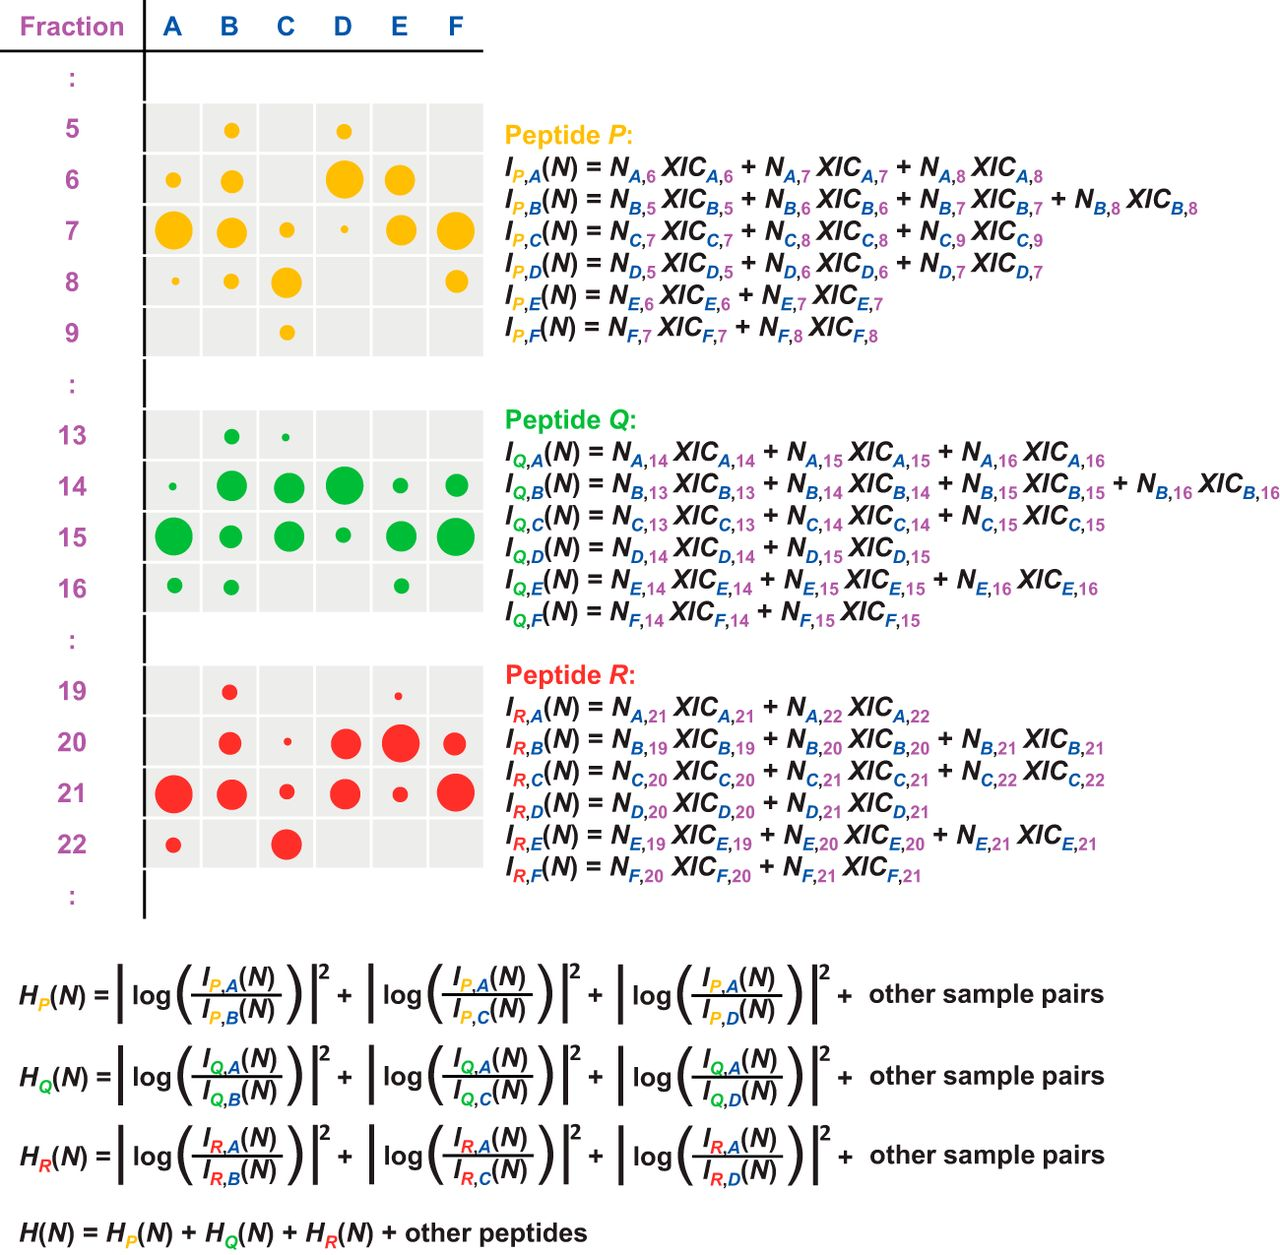
\includegraphics[width=0.8\textwidth]{xic_normalization}
\caption{Taken from \cite{Cox2014}}
\label{figure:xic_normalization}
\end{figure}


\subsubsection{Protein intensity inference}

Second, once the peptide intensities have been summarised, the intensity of the proteins that the peptides originated from are inferred. This is achieved in three steps (see figure \ref{figure:protein_quant_inference} for a graphical explanation).

\begin{enumerate}
\item Peptide intensity ratios are computed for all possible pairwise combinations by dividing the normalized intensities obtained in the previous step.

\item For every inferred protein A, its protein ratio $r_{A, a,b}$ for the pair of samples a,b is set to the median intensity of its children peptide ratio in samples a,b. The median is selected as a summarising statistic to protect from outliers. A minimal number of non-zero intensity peptides are required for the median to be valid, usually 2. Otherwise, the protein ratio for the pair of samples is set to 0.

\item The correct protein intensities are assumed to minimise the sum of the squared difference of the logarithm of the protein ratios and logarithm of the protein intensities $I$.

\end{enumerate}

\begin{equation}\label{eq:least_squares}
\sum_{a,b} (\log{(r_{A, a,b})} - \log{(I_{A,a})} + \log{(I_{A,b})})^2
\end{equation}

\begin{figure}[!h]
\centering
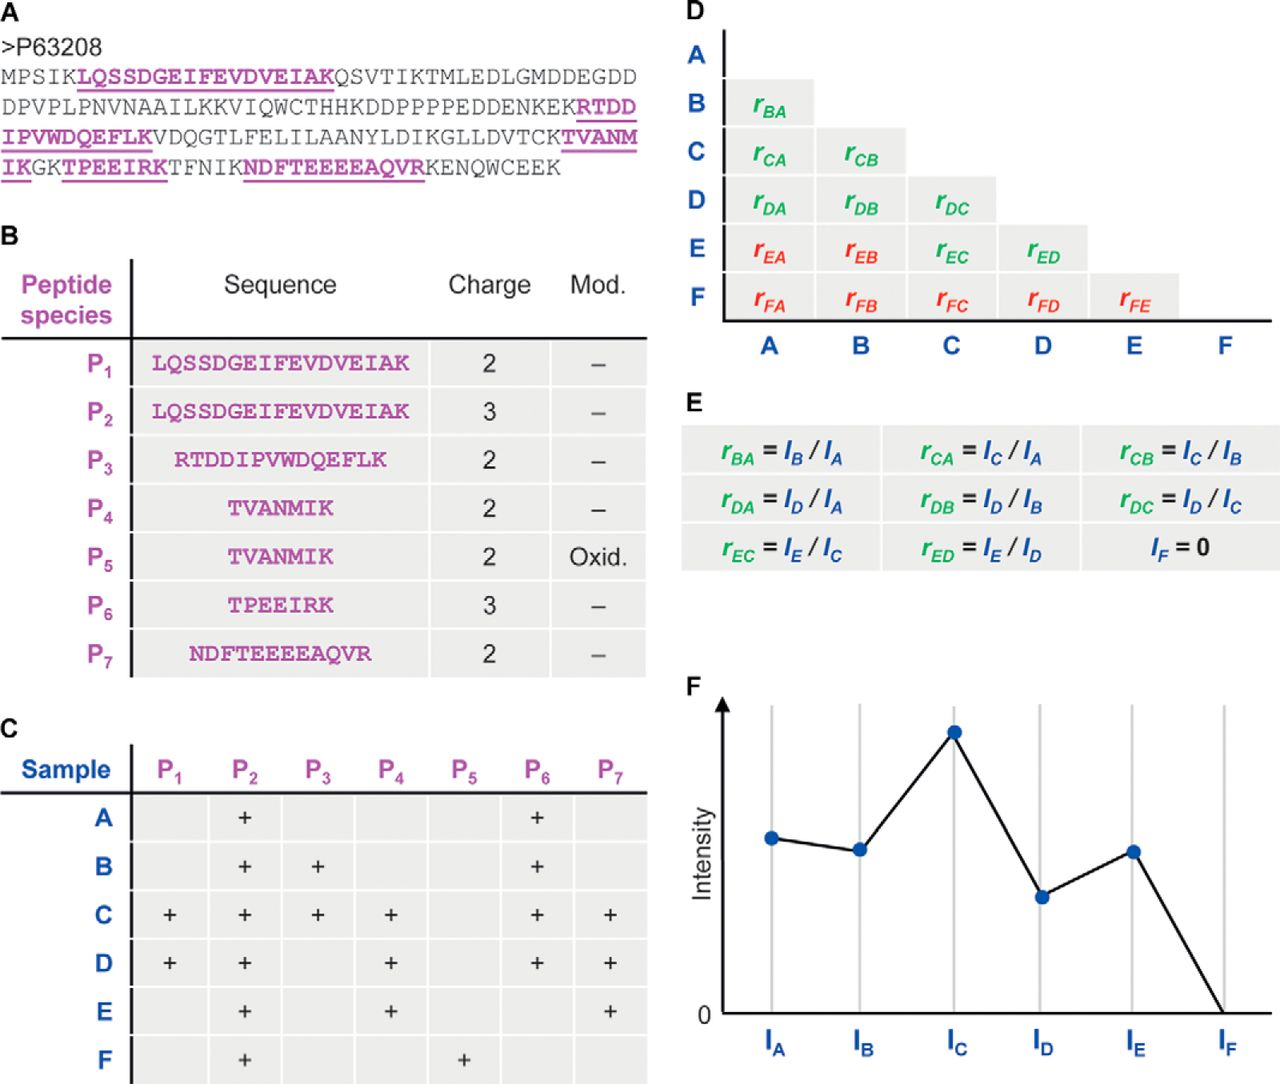
\includegraphics[width=0.8\textwidth]{protein_quant_inference}
\caption{Taken from \cite{Cox2014}}
\label{figure:protein_quant_inference}
\end{figure}

For the three most intense tryptic peptides, the signal per mole of protein was shown to be constant within a coefficient of variation of $\pm 10 \%$ \cite{Mikalsen2007}. Thus, protein intensities are linearly proportional to protein quantities and protein quantity ratios can be computed from protein intensity ratios. These values are reported in the MaxQuant output in the \texttt{proteinGroups.txt} file under columns named \textit{LFQ Intensity}.
		
\subsubsection{Drawbacks of the model}

The LFQ model provides a powerful method to infer protein quantities from a label-free experiment. However, it makes use of point estimates in different steps of the process, namely (1) during peptide intensity aggregation, where the Levenberg-Marquardt minimum is selected (2) during protein ratio estimation, where the peptide median is selected and (3) during protein intensity estimation, where the least squares minimum is selected. These point estimation bottlenecks, specially (2), discard increasing amounts of data that could otherwise be used for more accurate results. Moreover, not just quantities, but also the uncertainty behind them, could also be provided. The only way of MaxQuant to provide uncertainty measurements is the number of peptides supporting the quantification measurement.


\subsection{Bayesian model}

Bayesian statistics provides probability measurements for observed data assuming underlying mathematical models. A model for protein quantification based on the \ac{MS1} intensities or XICs could be developed to assess both quantities and uncertainties behind the estimated quantities.

While \ac{MS1} intensity measurements are dependent upon the underlying protein quantities, other factors influence the final measurement, thus adding noise and distorting the results. Besides the actual quantity, two more factors can be distinguished:

\begin{itemize}

\item \textbf{Sequence derived factors}: some peptides are easier to cleave for the cleaving enzyme (Trypsin, etc) than others. Moreover, the sequence of the peptide could influence the final measurement detected in the analyzer, by having different elution dynamics in the column or the analyzer.

\item \textbf{Random noise}: the stochastic processes intrinsic to \ac{MS1} measurements could also have an impact.

\end{itemize}

The model would take as input:

\begin{enumerate}

\item \textbf{Features extracted from the precursor sequence}, including the surrounding aminoacids in the original protein. They can be used to model the sequenced derived factors.

\item \textbf{Observed \ac{MS1} precursor intensities/XICs}.

\end{enumerate}

and return as output a protein quantification value for each protein, together with a measurement of the uncertainty behind it.




\subsection{Data}

The MaxLFQ paper dataset is available \footnote{\href{https://www.ebi.ac.uk/pride/archive/projects/PXD000279}{https://www.ebi.ac.uk/pride/archive/projects/PXD000279}}. The authors submitted the RAW files (>50 GB) and the search files containing the final results. They can be used to benchmark any new quantification tool or method, for example, it has been used to benchmark third party quantification tools like StPeter from the TPP \cite{Hoopmann2018}.

The dataset contains the results of the quantification of proteins in 2 different proteomes (\textit{E. coli} and \textit{Homo sapiens}) from 6 samples organized in 2 conditions with 3 replicates each. In the first condition (H), both proteomes were mixed in a 1:1 ratio, while in the second condition (L), the \textit{E. coli} proteome had 3 times more contribution to the mix (3:1). Thus, the fold change of protein quantities across conditions should be 1 for human proteins and 3 for bacterial proteins.

A list of the protein groups identified that could be mapped unambiguously to each species was made available \footnote{\href{http://www.mcponline.org/content/13/9/2513/suppl/DC1}{http://www.mcponline.org/content/13/9/2513/suppl/DC1}}. Thus, a dataset of thousands of proteins of known ratios between conditions, producing tens of thousands of peptides with known sequence, \ac{MS1} intensity/XIC and parent protein can be built from the publication, and used to train new quantification methods (figure \ref{fig:screenshot_peptide_data}).

% latex table generated in R 3.4.3 by xtable 1.8-2 package
% Fri Jun 01 17:11:23 2018
\begin{table}[ht]
\centering
\begin{tabular}{rlrr}
  \hline
 & Taxonomy & Peptides & Proteins \\ 
  \hline
1 & Escherichia coli (strain K12) & 14483 & 1556 \\ 
  2 & Homo sapiens & 32647 & 3444 \\ 
   \hline
   & Total & 47130 & 5000
\end{tabular}
\caption{Summary table of the dataset}
\label{table:summary_peptide_data}
\end{table}

\begin{figure}[!h]
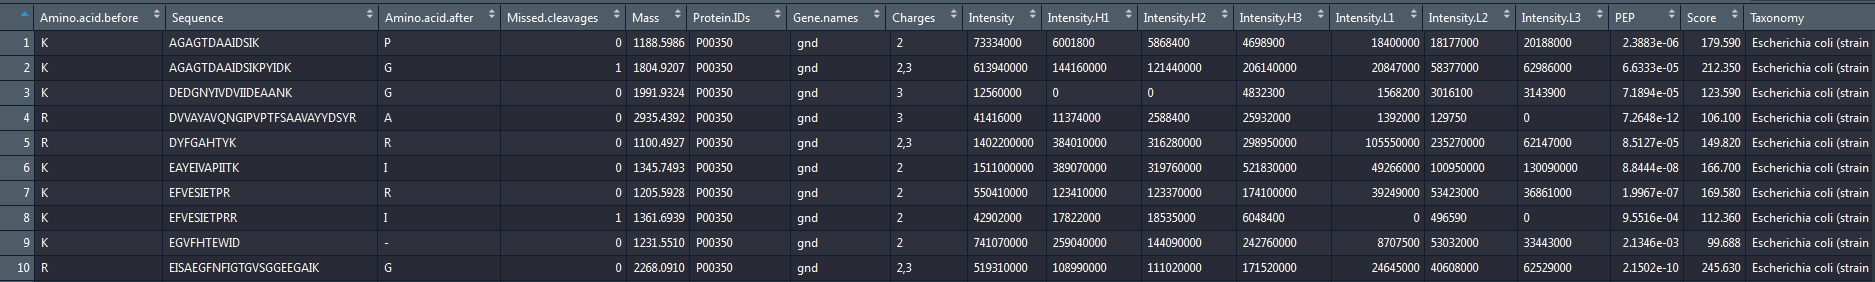
\includegraphics[width=1\textwidth]{dataset}
\caption{Extract of the available dataset. Total of 47130 entries, one per peptide, for a global of 5000 proteins.}
\label{fig:screenshot_peptide_data}
\end{figure}

This compiled dataset can be downloaded here \href{https://mega.nz/\#!AgcTgJYa!w9DoAKYRc6u-SaRy\_UIMz3aileUHXoaWgrxf-UycqiQ}{https://mega.nz/\#!AgcTgJYa!w9DoAKYRc6u-SaRy\_UIMz3aileUHXoaWgrxf-UycqiQ}

\section{Extension of pipelines}

The Compomics suite of programmes provides the best documented and accesible set of tools for proteomics analysis, but still lacks proper quantification tools. The implementation of a MS1 intensity-based downstream quantification tool compatible with the output of the Compomics tools would yield a free Linux compatible, CLI supported, complete proteomics pipeline featuring a robust quantification method.

\bibliographystyle{unsrt_etal}
\footnotesize{\bibliography{bibliography}}

\end{document}
%%  ==================================================================
%%  End document

